\documentclass{beamer}
\usepackage[german, english]{babel}
\usepackage[utf8]{inputenc}
%\usepackage{hyperref}
\usepackage{graphicx}
\usepackage{listings}
\usepackage{color}
%\usepackage{amsmath}

\definecolor{dkgreen}{rgb}{0,0.6,0}
\definecolor{gray}{rgb}{0.5,0.5,0.5}
\definecolor{mauve}{rgb}{0.58,0,0.82}
\definecolor{red}{rgb}{0.8,0.1,0.2}

\lstset{ %
	language=c,                % the language of the code
	basicstyle=\footnotesize\ttfamily,       % the size of the fonts that are used for the code
	numbers=left,                   % where to put the line-numbers
	numberstyle=\color{gray},  % the style that is used for the line-numbers
	                                % will be numbered
	numbersep=5pt,                  % how far the line-numbers are from the code
  backgroundcolor=\color{white},      % choose the background color. You must add \usepackage{color}
	showspaces=false,               % show spaces adding particular underscores
	showstringspaces=false,         % underline spaces within strings
	showtabs=false,                 % show tabs within strings adding particular underscores
	tabsize=2,                      % sets default tabsize to 2 spaces
	breaklines=true,                % sets automatic line breaking
	breakatwhitespace=true,        % sets if automatic breaks should only happen at whitespace
	keywordstyle=\bfseries\color{dkgreen},
	commentstyle=\itshape\color{gray},
	stringstyle=\color{mauve},         % string literal style
}

\title{Show and Tell}
\author{Daniel Pollack}

\begin{document}

\begin{frame}
	\maketitle
\end{frame}

\begin{frame}
	\tableofcontents
\end{frame}

\begin{frame}
	\frametitle{Pers. Daten}
	\section{Pers. Daten}

	\centering
	\begin{tabular}{ll}
		Name & Daniel Pollack\\
		Studiengang & Medieninformatik (Bachelor)\\
		Fachsemester & 6.
	\end{tabular}
\end{frame}

\begin{frame}
	\frametitle{Mack the Knife}
	\section{Mack the Knife}

	\begin{itemize}
	  \item Was ist Mack the Knife?
	    \begin{itemize}
	     \item Ein modulares Passwort Wiederherstellungs-Framework, dass hauptsächlich die Grafikkarte nutzt.
	     \item Nutzt CUDA und C++
	    \end{itemize}
	  \item Wann?
	    \begin{itemize}
	     \item vergangenes Semester (WS2012/13)
	    \end{itemize}
	\end{itemize}
\end{frame}

\begin{frame}
	\frametitle{MPD Interface für den Raspberry Pi}
	\section{MPD Interface für den Raspberry Pi}

	\begin{itemize}
	 \item Motivation:
	  \begin{itemize}
	   \item Ein Interface zur vereinfachten Bedienung des MPD (Music Player Daemon) für meine Mitbewohner
	  \end{itemize}
	 \item Umsetzung:
	  \begin{itemize}
	    \item Verknüpfung des Raspberry Pi via GPIO Schnittstelle mit einer Platine bestehend aus einem LCD Display und 5 Buttons
	    \item Geeignete Bibliothek für die MPD Steuerung unter Python finden
	    \item Python Script für die MPD - LCD Schnittstelle schreiben
	    \item Bugs fixen
	  \end{itemize}
	\end{itemize}
\end{frame}

\begin{frame}
  \frametitle{MPD Interface für den Raspberry Pi}
  \centering
  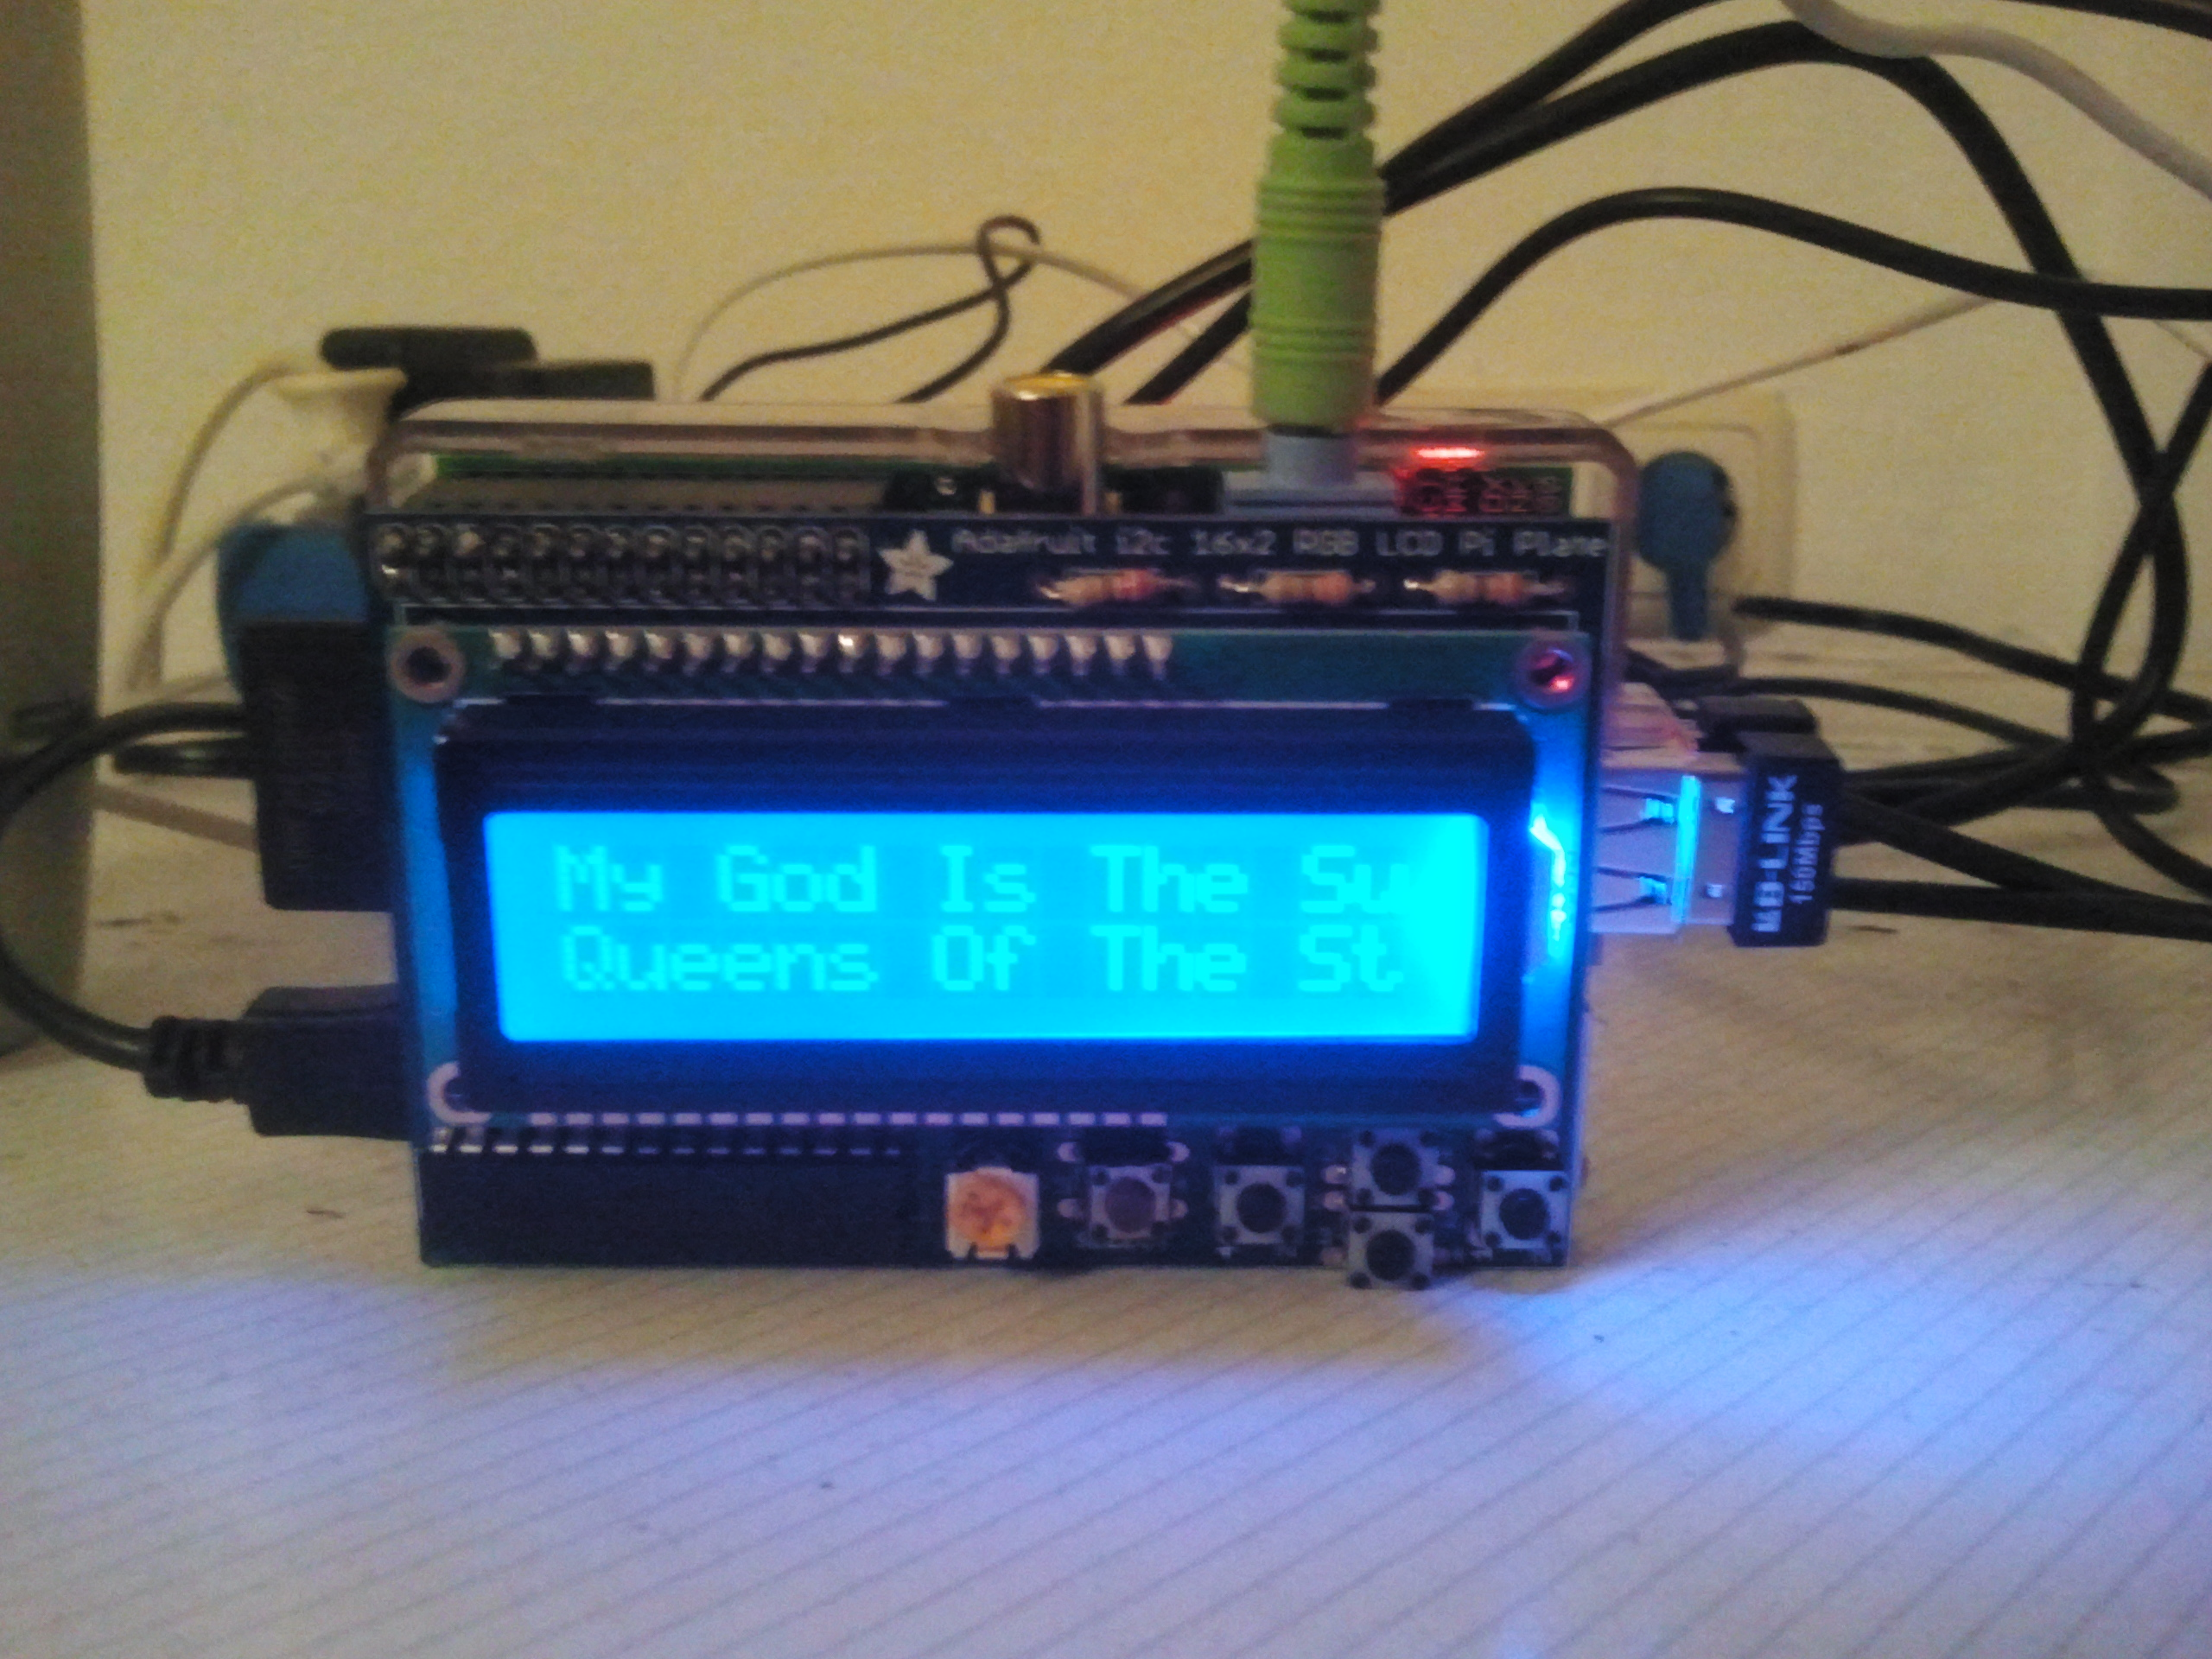
\includegraphics[bb=0 0 2560 1920,scale=0.1,keepaspectratio=true]{./pic/01.jpg}
  % 2013-04-08 21.14.27.jpg: 2560x1920 pixel, 72dpi, 90.31x67.73 cm, bb=0 0 2560 1920
\end{frame}

\end{document}
